% !TeX program = xelatex
% Сборка: xelatex report.tex
% Все персональные данные для титульного листа изменяются в этом блоке.
\documentclass[14pt,a4paper]{extarticle}

\usepackage{graphicx}
\usepackage{listings}
\usepackage{amsmath}
\usepackage{fontspec}
\IfFontExistsTF{Times New Roman}
    {
        \setmainfont{Times New Roman}
        \setsansfont{Times New Roman}
        \setmonofont{Times New Roman}
        \newfontfamily\cyrillicfont{Times New Roman}
        \newfontfamily\cyrillicfontsf{Times New Roman}
        \newfontfamily\cyrillicfonttt{Times New Roman}
    }
    {
        \setmainfont{Liberation Serif}
        \setsansfont{Liberation Serif}
        \setmonofont{Liberation Serif}
        \newfontfamily\cyrillicfont{Liberation Serif}
        \newfontfamily\cyrillicfontsf{Liberation Serif}
        \newfontfamily\cyrillicfonttt{Liberation Serif}
        \PackageWarningNoLine{report}{Times New Roman is not installed;
        using Liberation Serif temporarily}
    }
\usepackage{unicode-math}
\setmathfont{texgyretermes-math.otf}
\usepackage{polyglossia}
\setdefaultlanguage{russian}
\usepackage[left=30mm,right=15mm,top=20mm,bottom=20mm]{geometry}
\usepackage{setspace}
\usepackage{indentfirst}
\usepackage{enumitem}
\usepackage{titlesec}
\usepackage{caption}
\usepackage{float}
\usepackage[section]{placeins}
\usepackage{tabularx}
\usepackage{tikz}
\usetikzlibrary{arrows.meta,positioning}
\usepackage{pgfplots}
\pgfplotsset{compat=1.18}
\usepackage[hidelinks]{hyperref}

\lstset{language=C,basicstyle=\rmfamily\normalsize,breaklines=true,columns=fullflexible,keepspaces=true,showstringspaces=false}
\newcommand{\Ministry}{МИНОБРНАУКИ РОССИИ}
\newcommand{\University}{Санкт-Петербургский государственный\\
электротехнический университет\\
«ЛЭТИ» им. В.И. Ульянова (Ленина)}
\newcommand{\Department}{Название кафедры}
\newcommand{\StudentName}{Фамилия И.~О.}
\newcommand{\StudentGroup}{0000}
\newcommand{\TeacherName}{Фамилия И.~О.}
\newcommand{\City}{Санкт-Петербург}

\setstretch{1.5}
\setlength{\parindent}{1.25cm}
\setlength{\parskip}{0pt}
\setlength{\emergencystretch}{3em}
\titleformat{\section}{\normalfont\bfseries\centering}{\thesection}{0.5em}{}
\titlespacing*{\section}{0pt}{1.5em}{1em}
\titleformat{\subsection}{\normalfont\bfseries}{\thesubsection.}{0.5em}{}
\setlist{nosep,leftmargin=1.25cm}
\captionsetup{
    font=normalsize,
    labelsep=endash,
    skip=6pt
}
\captionsetup[figure]{
    name=Рисунок,
    justification=centering,
    singlelinecheck=false
}
\captionsetup[table]{
    name=Таблица,
    position=top,
    justification=raggedright,
    singlelinecheck=false
}
\newcommand{\sectionbreak}{\clearpage}

\begin{document}

\begin{titlepage}
    \thispagestyle{empty}
    \begin{center}
        \Ministry

        \University

        Кафедра \Department
    \end{center}

    \vspace{2cm}

    \begin{center}
        \textbf{ОТЧЕТ}

        по практической работе №~1

        по дисциплине «Системы параллельной обработки сигналов»

        \vspace{0.5cm}
        Тема: «Запуск параллельной программы на различном числе
        одновременно работающих процессов. Упорядочение вывода результатов»
    \end{center}

    \vspace{2cm}

    \begin{flushright}
        \begin{minipage}{0.8\textwidth}
            \begin{tabularx}{\linewidth}{@{}p{4.8cm}
                >{\centering\arraybackslash}p{2.8cm} X@{}}
                Студент гр. \StudentGroup
                & \rule{2.5cm}{0.4pt} & \StudentName\\
                & подпись & \\[0.8cm]
                Преподаватель
                & \rule{2.5cm}{0.4pt} & \TeacherName\\
                & подпись &
            \end{tabularx}
        \end{minipage}
    \end{flushright}

    \vfill

    \begin{center}
        \City\\
        2026
    \end{center}
\end{titlepage}

\setcounter{page}{2}

\section{Цель работы}

Познакомиться с запуском MPI-программы на различном числе процессов,
обменом сообщениями между процессами и способами управления порядком вывода
результатов параллельного выполнения.

\section{Формулировка задания}

Отдельный номер варианта в исходном задании не задан; работа
выполнена по единственной предложенной формулировке.

\textbf{Задание 1.} Все процессы, кроме процесса с рангом 0, передают
значение своего ранга нулевому процессу. Процесс с рангом 0 сначала печатает
значение собственного ранга, затем принимает сообщения с рангами остальных
процессов и также выводит их. Порядок приёма сообщений заранее не определён и
может изменяться от запуска к запуску.

Необходимо несколько раз запустить программу при фиксированном числе
процессов (например, при восьми), проанализировать порядок вывода сообщений и
сформулировать правило, которое его определяет.

\textbf{Задание 2.} Модифицировать программу так, чтобы порядок вывода
сообщений соответствовал номерам процессов. Сравнить результаты работы двух
вариантов программы.

\section{Описание алгоритмов}

Реализован вариант задания 1 на языке C с MPI. Все $p$ процессов вызывают
\texttt{MPI\_Init}, определяют ранг и число процессов. Каждый процесс с
рангом $i>0$ отправляет одно целое число $i$ процессу 0 с тегом 0.
Процесс 0 печатает собственный ранг и выполняет ровно $p-1$ операций
\texttt{MPI\_Recv} с источником \texttt{MPI\_ANY\_SOURCE}, печатая
полученное значение и фактического отправителя из \texttt{MPI\_Status}.
Все процессы завершают работу через \texttt{MPI\_Finalize}.

При проверке исправлена граница цикла: ранее выполнялось $p$ приёмов,
хотя отправлялось только $p-1$ сообщений. Лишний приём приводил к зависанию.
При $p=1$ исправленная программа только печатает ранг 0 и завершается.

Для задания 2 создана отдельная программа. В цикле по
$i=1,\ldots,p-1$ источником приёма указывается процесс $i$ вместо
\texttt{MPI\_ANY\_SOURCE}. Все отправители работают параллельно. Процесс 0
по очереди ожидает сообщения от процессов 1, 2, \ldots, $p-1$ и тем самым
задаёт порядок печати.

\section{Формальное описание с помощью сетей Петри}

Используется параметризованная сеть Петри с цветными фишками. Формализация
выполнена с опорой на основные положения аппарата сетей Петри~[1].
Для каждого $i\in\{1,\ldots,p-1\}$ место $A_i$ содержит одну начальную
фишку готовности отправителя, $B_i$ обозначает завершение его обмена.
Место $R$ содержит фишку состояния принимающего процесса $(k,L)$:
число принятых сообщений и последовательность уже напечатанных рангов.
Начальное место $Z$ содержит одну фишку готовности процесса 0.
Место $F$ обозначает завершение приёма.

Переход $t_0:Z\to R$ печатает 0 и создаёт фишку $(0,[0])$.
Для каждого $i>0$ переход обмена имеет входы $A_i,R$ и выходы $B_i,R$:
\begin{equation}
\label{eq:petri-transition}
 A_i+R(k,L)\xrightarrow{t_i}B_i+R(k+1,L\mathbin{\|}[i]).
\end{equation}
Выражение~\eqref{eq:petri-transition} задаёт функционал $t_i$: передать
ранг $i$, принять его процессом 0 и напечатать.
Обмен отправителя с получателем здесь моделируется одним совместным
переходом; внутренняя буферизация MPI абстрагирована.
В неупорядоченном варианте допустим любой ещё не сработавший $t_i$.
В упорядоченном варианте дополнительное условие перехода: $i=k+1$.
Переход $t_f:R\to F$ разрешён только при $k=p-1$; он завершает фазу приёма.

Каждый $t_i$ срабатывает ровно один раз, поскольку фишка $A_i$ имеется
в одном экземпляре. Фишка $R$ задаёт последовательную печать процессом 0.
Итоговый список содержит все ранги ровно по одному разу.
При $p=1$ после $t_0$ сразу разрешён $t_f$.

Графическая схема параметризованной сети представлена на
рисунке~\ref{fig:petri-net}.

\begin{figure}[H]
    \centering
    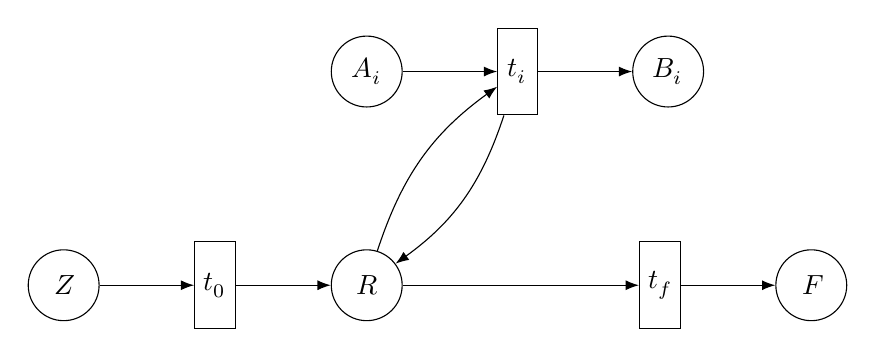
\begin{tikzpicture}[
        >=Latex,
        place/.style={circle,draw,minimum size=9mm},
        transition/.style={rectangle,draw,minimum width=5mm,minimum height=11mm},
        node distance=12mm and 12mm
    ]
        \node[place] (z) {$Z$};
        \node[transition,right=of z] (t0) {$t_0$};
        \node[place,right=of t0] (r) {$R$};
        \node[transition,right=30mm of r] (tf) {$t_f$};
        \node[place,right=of tf] (f) {$F$};
        \node[place,above=18mm of r] (ai) {$A_i$};
        \node[transition,right=of ai] (ti) {$t_i$};
        \node[place,right=of ti] (bi) {$B_i$};

        \draw[->] (z) -- (t0);
        \draw[->] (t0) -- (r);
        \draw[->] (r) -- (tf);
        \draw[->] (tf) -- (f);
        \draw[->] (ai) -- (ti);
        \draw[->] (ti) -- (bi);
        \draw[->] (r) to[bend left=18] (ti);
        \draw[->] (ti) to[bend left=18] (r);
    \end{tikzpicture}
    \caption{Параметризованная сеть Петри для обмена сообщениями}
    \label{fig:petri-net}
\end{figure}

Графическая схема на рисунке~\ref{fig:petri-net} показывает один из
$p-1$ однотипных каналов отправителей. Дуги между $R$ и $t_i$
отражают изменение состояния принимающего процесса после каждого
сообщения.

\section{Реализация и функциональная проверка}

Полный листинг программы с неупорядоченным приёмом приведён в приложении А,
листинг программы с упорядоченным приёмом --- в приложении Б.

\subsection{Ход выполнения задания 1}

Программа собрана средствами CMake. Цель \texttt{task1\_unordered}
компилируется как программа на языке C11 и связывается с библиотекой MPI.
Для компиляторов GNU и Clang включены предупреждения \texttt{-Wall},
\texttt{-Wextra} и \texttt{-Wpedantic}. Сборка завершилась без ошибок.

После инициализации MPI каждый процесс определяет свой ранг. Процессы с
рангами больше нуля передают свои номера процессу 0. Нулевой процесс сначала
выводит 0, затем выполняет $p-1$ операций \texttt{MPI\_Recv}. В каждой
операции источник задан константой \texttt{MPI\_ANY\_SOURCE}, поэтому может
быть принято сообщение от любого ещё не обслуженного отправителя.

Для начальной проверки программа запущена на одном и двух процессах. При
$p=1$ отправители отсутствуют, поэтому выводится только 0. При $p=2$
процесс 0 получает единственное сообщение от процесса 1. Результат сборки
и запусков представлен на рисунке~\ref{fig:task1-p1-p2}.

\begin{figure}[H]
    \centering
    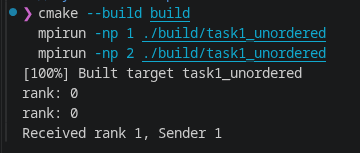
\includegraphics[width=0.72\linewidth]{screenshots/task1_build_p1_p2.png}
    \caption{Сборка и запуск неупорядоченной программы на одном и двух
    процессах}
    \label{fig:task1-p1-p2}
\end{figure}

Затем выполнено пять запусков при $p=8$. В каждом опыте программа
завершилась, нулевой ранг был напечатан первым, а каждый из рангов 1--7
встретился ровно один раз. Полученные последовательности приведены в
таблице~\ref{tab:task1-p8-sequences}.

\begin{table}[H]
\caption{Последовательности рангов в пяти запусках на восьми процессах}
\label{tab:task1-p8-sequences}
\centering
\begin{tabular}{c|l}
Запуск & Ранги в порядке печати \\
\hline
1 & 0, 7, 3, 5, 2, 6, 4, 1 \\
2 & 0, 2, 6, 7, 3, 4, 1, 5 \\
3 & 0, 1, 2, 3, 4, 5, 6, 7 \\
4 & 0, 1, 4, 2, 7, 3, 6, 5 \\
5 & 0, 7, 1, 3, 4, 5, 6, 2
\end{tabular}
\end{table}

Первым всегда печатается 0. Далее вывод соответствует порядку, в котором
операции приёма выбирают подходящие сообщения. Источник
\texttt{MPI\_ANY\_SOURCE} допускает приём от любого процесса, поэтому порядок
отправителей не задаётся. На результат влияют планирование процессов и работа
MPI; нельзя гарантировать ни возрастание рангов, ни порядок начала отправок,
ни строгую сортировку по времени физического прихода сообщений.
Одинаковые последовательности при повторных запусках тоже допустимы.
Передаются сообщения с целыми числами, а не сигналы ОС. Полный вывод пяти
запусков показан на рисунке~\ref{fig:task1-p8}.

\begin{figure}[H]
    \centering
    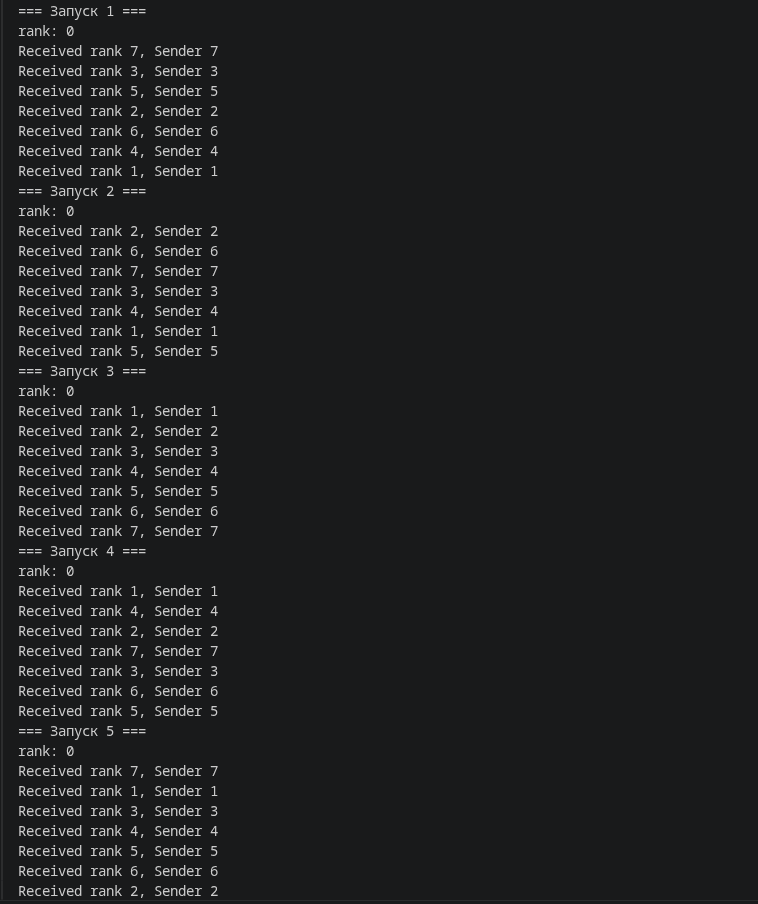
\includegraphics[width=0.83\linewidth]{screenshots/task1_p8_runs_full.png}
    \caption{Пять запусков неупорядоченной программы на восьми процессах}
    \label{fig:task1-p8}
\end{figure}

\subsection{Ход выполнения задания 2}

Вторая программа получена изменением источника в операции
\texttt{MPI\_Recv}: вместо произвольного отправителя
\texttt{MPI\_ANY\_SOURCE} используется значение счётчика цикла $i$.
Алгоритм отправителей и количество операций приёма остались без изменений.
Таким образом, на первой итерации процесс 0 ожидает сообщение от процесса 1,
на второй --- от процесса 2 и далее до процесса $p-1$. Сообщение от процесса
с большим рангом может быть готово раньше, но будет обработано только после
всех отправителей с меньшими рангами.

Программа собрана средствами CMake и сначала проверена при $p=1,2,4$.
При одном процессе выводится только 0; при двух и четырёх процессах получены
строго возрастающие последовательности рангов
(рисунок~\ref{fig:task2-p1-p2-p4}).

\begin{figure}[H]
    \centering
    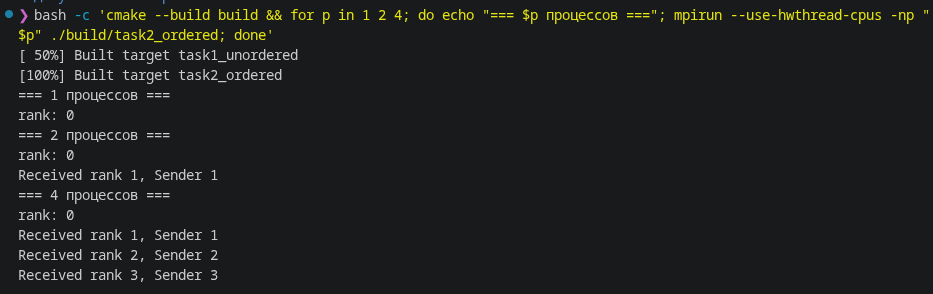
\includegraphics[width=0.95\linewidth]{screenshots/task2_build_p1_p2_p4.png}
    \caption{Сборка и запуск упорядоченной программы на одном, двух и четырёх
    процессах}
    \label{fig:task2-p1-p2-p4}
\end{figure}

Для проверки устойчивости результата выполнены три запуска при $p=8$.
Во всех запусках получена одна последовательность
$0,1,2,3,4,5,6,7$, что подтверждает заданный программой порядок приёма.
Результаты повторных запусков представлены на рисунке~\ref{fig:task2-p8}.

\begin{figure}[H]
    \centering
    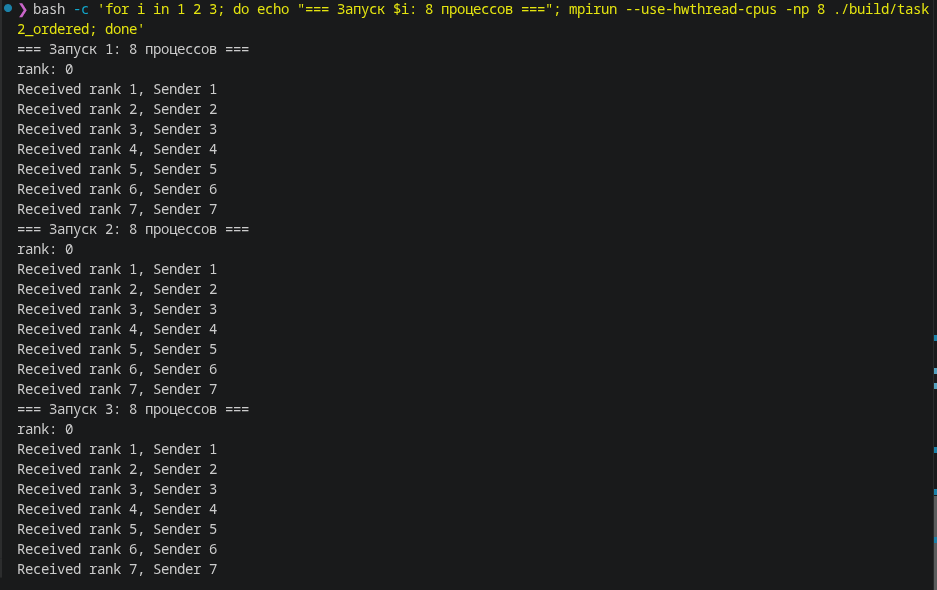
\includegraphics[width=0.9\linewidth]{screenshots/task2_p8_runs.png}
    \caption{Три запуска упорядоченной программы на восьми процессах}
    \label{fig:task2-p8}
\end{figure}

Дополнительно выполнен функциональный запуск при $p=16$. Поскольку
используемый процессор предоставляет 12 аппаратных потоков, применён параметр
\texttt{--oversubscribe}. Этот опыт подтверждает корректность порядка
$0,1,\ldots,15$, но из-за переподписки не используется для оценки
производительности. Результат показан на рисунке~\ref{fig:task2-p16}.

\begin{figure}[H]
    \centering
    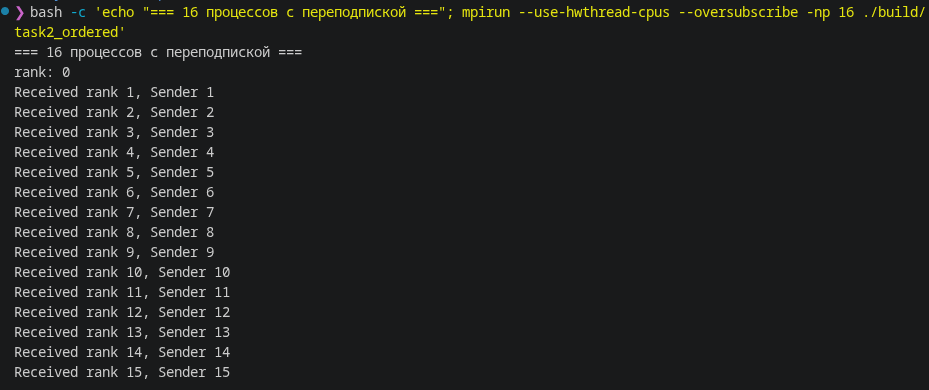
\includegraphics[width=0.95\linewidth]{screenshots/task2_p16.png}
    \caption{Запуск упорядоченной программы на шестнадцати процессах с
    переподпиской}
    \label{fig:task2-p16}
\end{figure}

\section{Экспериментальное исследование}

\subsection{Методика измерения}

Для неупорядоченного алгоритма создана экспериментальная программа,
листинг которой приведён в приложении В. Параметр $n$ задаёт число
целых чисел в сообщении каждого отправителя. Исследованы размеры
$n=1$, 1024 и 65536, что соответствует 4 байтам, 4 Кбайт и 256 Кбайтам.

Заполнение буфера выполнялось до начала замера. Все процессы
синхронизировались вызовом \texttt{MPI\_Barrier}, после чего на каждом
процессе фиксировалось начало и окончание обмена функцией
\texttt{MPI\_Wtime}. За время опыта принимался максимум локальных времён,
полученный через \texttt{MPI\_Reduce} с операцией \texttt{MPI\_MAX}.
Печать в измеряемый участок не входила.

Для каждой пары $(p,n)$ выполнен один прогревочный и пять измерительных
запусков; итоговым значением считалась медиана. Использованы
$p=1,2,4,8,16$. Измерения проводились на Intel Core i5-12400F
(шесть ядер, 12 аппаратных потоков) под Linux 7.3.0-4-cachyos с
Open~MPI 5.0.11. Программа собиралась GCC 16.2.1 в режиме Release.
При $p=16$ использован параметр \texttt{--oversubscribe}, поэтому этот режим
отмечен как переподписка.

\subsection{Результаты неупорядоченного приёма}

Сводный вывод сценария измерений представлен на
рисунке~\ref{fig:task1-benchmark-summary}, а медианы переведены в микросекунды и
приведены в таблице~\ref{tab:task1-timing}.

\begin{figure}[H]
    \centering
    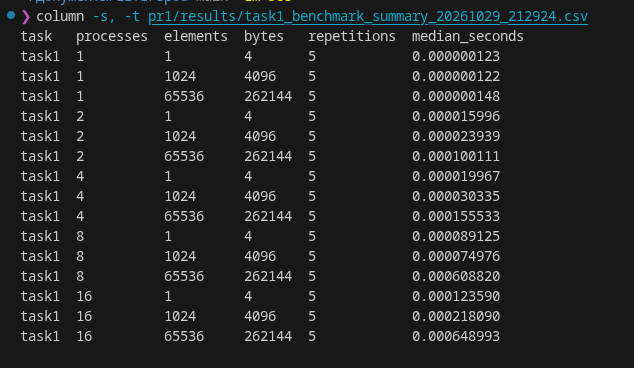
\includegraphics[width=0.98\linewidth]{screenshots/task1_benchmark_summary.png}
    \caption{Сводные результаты измерений для задания 1}
    \label{fig:task1-benchmark-summary}
\end{figure}

\begin{table}[H]
\caption{Медианное время неупорядоченного обмена}
\label{tab:task1-timing}
\centering
\begin{tabular}{c|c|c|c}
$p$ & $T(n=1)$, мкс & $T(n=1024)$, мкс & $T(n=65536)$, мкс \\
\hline
1  & 0,123   & 0,122   & 0,148 \\
2  & 15,996  & 23,939  & 100,111 \\
4  & 19,967  & 30,335  & 155,533 \\
8  & 89,125  & 74,976  & 608,820 \\
16 & 123,590 & 218,090 & 648,993
\end{tabular}
\end{table}

На рисунке~\ref{fig:task1-time-processes} показана зависимость времени от числа
процессов. Контрольные точки $p=1$ не включены, поскольку обмен
в них отсутствует.

\begin{figure}[H]
\centering
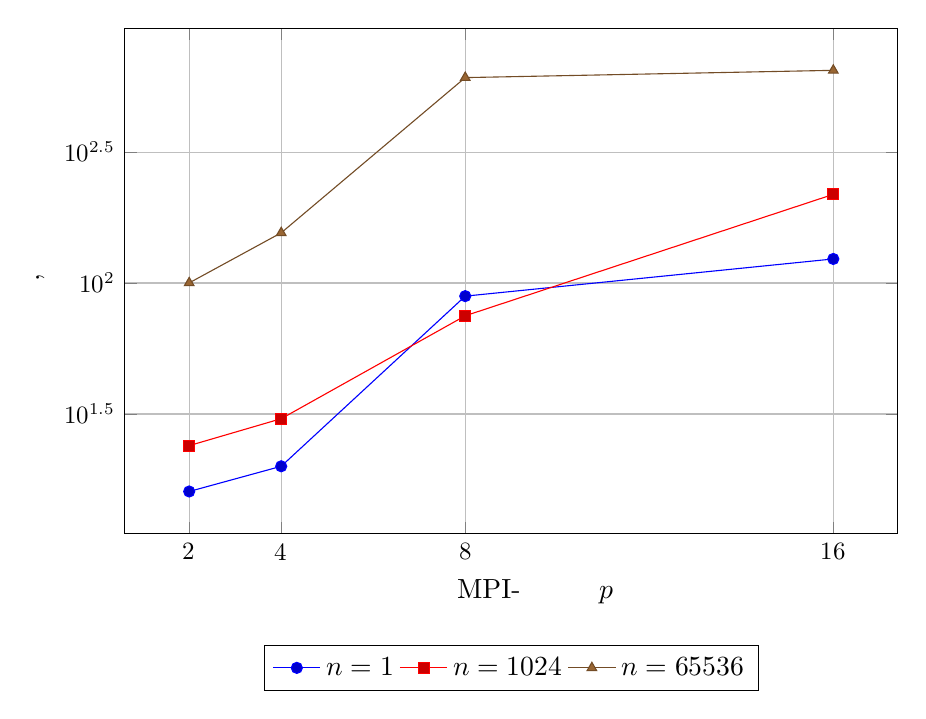
\begin{tikzpicture}
\begin{axis}[
    width=0.94\linewidth,
    height=8cm,
    xlabel={Число MPI-процессов $p$},
    ylabel={Время, мкс},
    xtick={2,4,8,16},
    ymode=log,
    grid=major,
    legend style={at={(0.5,-0.22)},anchor=north,legend columns=3},
    tick label style={font=\small}
]
\addplot+[mark=*] coordinates {(2,15.996) (4,19.967) (8,89.125) (16,123.590)};
\addlegendentry{$n=1$}
\addplot+[mark=square*] coordinates {(2,23.939) (4,30.335) (8,74.976) (16,218.090)};
\addlegendentry{$n=1024$}
\addplot+[mark=triangle*] coordinates {(2,100.111) (4,155.533) (8,608.820) (16,648.993)};
\addlegendentry{$n=65536$}
\end{axis}
\end{tikzpicture}
\caption{Зависимость времени неупорядоченного обмена от числа процессов}
\label{fig:task1-time-processes}
\end{figure}

Влияние размера сообщения показано на рисунке~\ref{fig:task1-time-size}.
Для больших буферов рост времени выражен сильнее, чем для единичного
сообщения.

\begin{figure}[H]
\centering
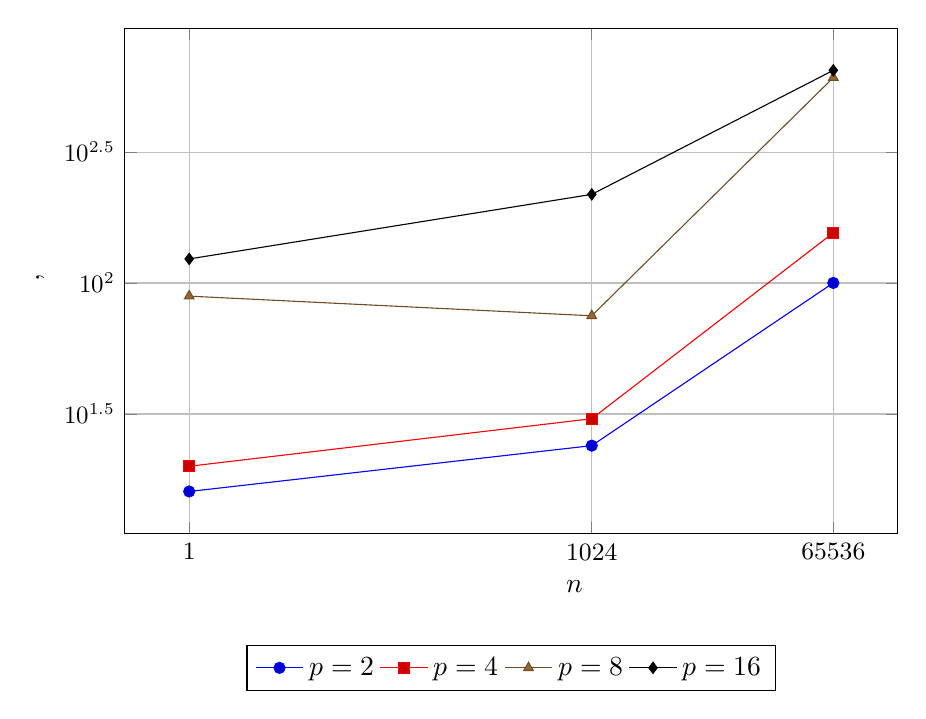
\begin{tikzpicture}
\begin{axis}[
    width=0.94\linewidth,
    height=8cm,
    xlabel={Число элементов $n$},
    ylabel={Время, мкс},
    xmode=log,
    ymode=log,
    xtick={1,1024,65536},
    xticklabels={1,1024,65536},
    grid=major,
    legend style={at={(0.5,-0.22)},anchor=north,legend columns=4},
    tick label style={font=\small}
]
\addplot+[mark=*] coordinates {(1,15.996) (1024,23.939) (65536,100.111)};
\addlegendentry{$p=2$}
\addplot+[mark=square*] coordinates {(1,19.967) (1024,30.335) (65536,155.533)};
\addlegendentry{$p=4$}
\addplot+[mark=triangle*] coordinates {(1,89.125) (1024,74.976) (65536,608.820)};
\addlegendentry{$p=8$}
\addplot+[mark=diamond*] coordinates {(1,123.590) (1024,218.090) (65536,648.993)};
\addlegendentry{$p=16$}
\end{axis}
\end{tikzpicture}
\caption{Зависимость времени неупорядоченного обмена от размера сообщения}
\label{fig:task1-time-size}
\end{figure}

При $p=2$ увеличение $n$ от 1 до 65536 привело к росту медианы с
15,996 до 100,111~мкс. Для $p=8$ и $n=65536$ получено 608,820~мкс,
что примерно в шесть раз больше значения при $p=2$. Это согласуется с
тем, что при фиксированном $n$ суммарный объём равен $(p-1)n$ целых
чисел. Немонотонность для малых сообщений, в частности 89,125~мкс
при $p=8$, $n=1$ и 74,976~мкс при $n=1024$, объясняется сопоставимыми
с полезной работой накладными расходами и вариативностью планирования.
Точки $p=16$ дополнительно искажены переподпиской.

\subsection{Ограничения интерпретации}

При $p=1$ отправители отсутствуют, поэтому полученные значения около
0,12~мкс отражают лишь накладные расходы таймера. Отношение
$T(1,n)/T(p,n)$ не является ускорением: при росте $p$ число отправителей и
общий объём передачи увеличиваются. Поэтому графики ускорения и
эффективности для данной постановки не строились.

На текущем этапе измерена только версия с \texttt{MPI\_ANY\_SOURCE}.
Для строгого сравнения необходимо провести ту же серию опытов для
упорядоченного приёма при тех же $(p,n)$; это следующий этап работы.

\section{Выводы}

В ходе работы реализованы и проверены два способа приёма MPI-сообщений.
Источник \texttt{MPI\_ANY\_SOURCE} не задаёт порядок вывода: в пяти запусках на
восьми процессах получены различные последовательности. Явный источник $i$
обеспечил возрастающий порядок $0,1,\ldots,p-1$ во всех функциональных
запусках.

Для неупорядоченного приёма выполнено измерение времени для трёх размеров
сообщения и $p=1,2,4,8,16$. При росте размера буфера и числа отправителей
время в целом увеличивалось. Для $n=65536$ оно возросло с 100,111~мкс при
$p=2$ до 608,820~мкс при $p=8$. Режим $p=16$ выполнялся с переподпиской,
поэтому его значения нельзя напрямую сравнивать с режимами без неё.

Полученные времена не описывают ускорение, так как при увеличении $p$
одновременно растёт общий объём передачи, а при $p=1$ обмен отсутствует.
Следующий этап --- измерить упорядоченную версию по той же методике и сравнить
алгоритмы при равных $(p,n)$.

\section{Список использованных источников}

\begin{enumerate}[label=\arabic*,leftmargin=1.25cm]
    \item Мараховский В.~Б., Розенблюм Л.~Я., Яковлев А.~В.
    Моделирование параллельных процессов. Сети Петри.
    СПб.: Профессиональная литература, 2014.
\end{enumerate}

\clearpage
\phantomsection
\section*{ПРИЛОЖЕНИЕ А\\Листинг программы с неупорядоченным приёмом}
\lstinputlisting{../src/task1_unordered.c}

\clearpage
\phantomsection
\section*{ПРИЛОЖЕНИЕ Б\\Листинг программы с упорядоченным приёмом}
\lstinputlisting{../src/task2_ordered.c}

\clearpage
\phantomsection
\section*{ПРИЛОЖЕНИЕ В\\Листинг программы измерения времени}
\lstinputlisting{../src/task1_benchmark.c}

\end{document}
